% !TeX root = ../main.tex

\chapter{详细设计与实现}
本章节是基于第四章概要设计的基础上,给出整个系统中的详细设计与实现,
主要内容包括仿真平台硬件平台构建和硬件模型建模的实现以及整个平台的仿真运行流程细节、设
计空间探索过程过程中训练集和多目标预测模型的生成以及对设计空间探索结果分析这些部分
的具体实现。

\section{仿真平台模块硬件平台构建模块的设计与实现}
TopLevel仿真平台是基于任务图的一个以Simpy引擎为仿真框架的仿真系统\cite{36}。
TopLevel仿真平台的设计与实现是整个系统实现部分的重中之重,而对仿真系统各个模
块的建模则是这部分工作的核心。
整个仿真系统通过解析输入的硬件配置文件,实例化硬件模块,通过总线将各个硬件
模块连接起来,形成整个仿真平台的硬件平台部分。任务图管理模块通过解
析输入的任务图,并根据触发关系链式的调度任务,将任务分配到具体的硬
件模型上执行。下面将详细阐述仿真平台硬件平台构建模块的功能实现及结构。

整个仿真平台的硬件平台部分从结构上可以抽象为一个自顶而下的一个树状结构,
所有具体的硬件模型实例都被视为该树状结构的最底端的叶子节点,所有的叶子节点(硬件模型实例)
都是由上层的节点(不同的子组件)分区管理,依次逐层向上。树的根节点即为仿真平台的
硬件平台部分。仿真平台的硬件平台的树状结构示意图如图5.1所示:

\begin{figure}
    \centering
    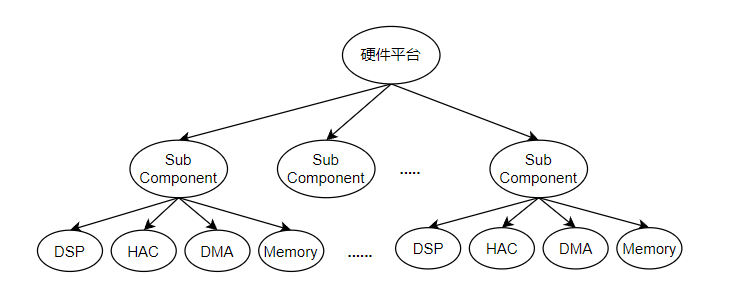
\includegraphics[width=1\textwidth]{硬件平台树状结构示意图.png}
    \caption{硬件平台树状结构示意图}
    \label{fig:badge}
\end{figure}

用户在进行仿真之前需要根据自己的需求去修改硬件平台配置文件,
硬件平台构建需要读取硬件平台配置文件并解析,系统所需的硬件平台配置文件包括
:V801.xml用来描述所有硬件模型之间的连接信息及Port信息、V801MemMap.xml
用来描述所有硬件模块模块与具体物理地址之间映射关系、V801MemPt.xml用来
描述内存模块的具体信息、V801Prop.xml用来描述所有需要实例化的模块包括
Processor和总线模块等等在实例化的时候的所需的所有具体信息、V801Route.xml
描述了所有实例化后的硬件模块之间的路由信息,将各个硬件模型通过总线连接形
成一个完整的硬件平台。在实际的用例仿真业务中,在进行用例仿真之前,仿真系统
先根据硬件平台配置文件对硬件平台进行构建。PlateformBuilder会实例化DSP、DMA
以及HAC等等硬件模型,当一个子组件中所有的硬件模块全部实例化后,再继续实例化
其他子组件中的硬件模块,最后当所有组件中硬件模块实例化成功后,整个仿真平台
的硬件平台就构建成功了。

我们通过创建SaeSimulator单实例去实现整个平台初始化的功能,整个SaeSimulator
的类图如图5.2所示:

\begin{figure}
    \centering
    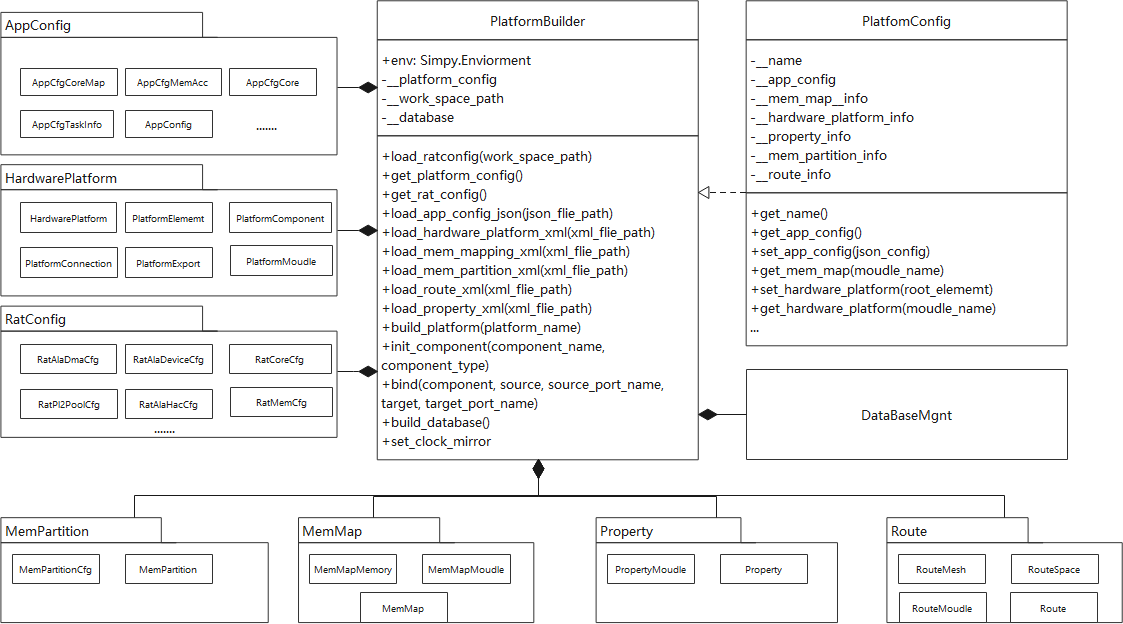
\includegraphics[width=1\textwidth]{硬件模块实例化模块类图.png}
    \caption{硬件模块实例化模块类图}
    \label{fig:badge}
\end{figure}

图5.2硬件平台实例化模块需要的类以及类之间关系构造的类图,在硬件平台实例化
模块中,我们在最外层通过SaeSimulator单实例调用load\_platform函数实现
PlatformBuilder类中对各个硬件配置文件的读取和解析以及实现硬件平台中
各个模型的实例化,PlatformBuilder类读取和解析硬件配置文件后,将硬件
配置信息存储到PlatformConfig类中各个属性中,并对每个属性设置get和
set函数,支持外部对类里面私有函数的设置和读取。最后,硬件模型的实
例化通过调用init\_component函数实现。

硬件模块实例化过程中,实现方式通过层次性的实例化。先按模块解析硬
件配置文件读取硬件配置信息。在逐层实例化各个模块。如硬件模块实例
化类图所示,每个包里是硬件的一部分,将包里的各个类根据读取的硬件
配置信息实例化,在实例化整个次外层的类,如AppConfig里的AppConfig
类。最后在init\_component函数中统一,最后通过bind函数将各个模块
通过路由信息中Port口连接起来。最后,通过DatabaseMgnt类实例化并
连接数据库文件。

\section{GeneralFifo模块设计与实现}

在整个仿真平台中,我们需要实现硬件模型能够在别的模块发送过来消息时
能够及时的对发送过来的消息进行处理,以及模型外部能够接收别的模型发
送过来消息的消息队列。这种消息队列主要用于Processor模块的流水线功能
的具体实现。

我们基于Simpy的事件机制实现了GeneralFifo模块,并在整体仿真平台构建
时将此模块作为基础数据结构使用,与先入先出队列的整体逻辑类似。我们
在概要设计中简要介绍了GeneralFifo的整体执行流程。我们在这一节详细
介绍GeneralFifo的设计。GeneralFifo模块的类图如图5.3所示:
\begin{figure}
    \centering
    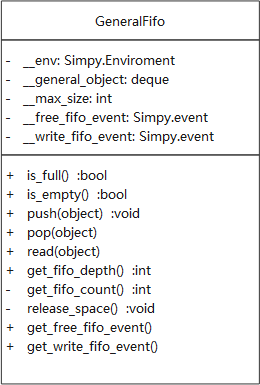
\includegraphics[width=0.45\textwidth]{GeneralFifo类图.png}
    \caption{GeneralFifo类图}
    \label{fig:badge}
\end{figure}

GeneralFifo模块的底层实现基于数据结构双向队列deque实现。整体实现
队列先入先出,并可以设置以及查询队列深度,查询队列中现有对象数量,
判断队列的状态。并基于Simpy的event机制实现了队列的Push和Pop功能。
每次将对象Push进队列时,将触发该队列的write\_fifo\_event,该event事
件触发时,会使在其他模块等待该事件触发的进程开始继续执行,从而实
现该队列一旦有对象存入,能够及时通知其他模块将对象从队列中取出进
行操作。同时,当队列为满时,其他模块只需等待free\_fifo\_event事件
触发,其他模块即可继续向Fifo中Push对象。这样就实现了不同模块之
间基于GeneralFifo的信息传输的功能,以及实现一个进程或者模块等待信息的
场景。在仿真平台中所有模块之间交互以及Processor模块的实现都是
基于GeneralFifo实现的。

\section{Processor模块设计与实现}

仿真平台中Processor模块主要功能为:接收调度器模块发送过来的任务实例并
提取任务实例中中的任务信息,在具体的硬件实例上根据任务信息处理任务。
Processor模型类型主要分为DSP模块、DMA模块和HAC模块。下面详细阐述了
仿真平台Processor相关模块设计与实现。

Processor模块主要实现对三种基础硬件模型(DSP、HAC和DMA)的建模
以及Processor模块与调度器模块之间的交互。在实现三种基础模型的
建模之前,我们实现ProcessorBase类,通过ProcessorBase类所有
Processor模型的基础功能进行实现。

平台中所有模型都是以GeneralModule类为基类实现,GeneralModule
模块是统一所有已实例化的模型并将这些模型联系起来的模块。GeneralModule
模块实现了平台信息和实际硬件模型信息的联系,并为每个模型模块创
建了Log文件,在各模块中可以调用其基类GeneralModule类中的log方
法去记录log信息,并统一设置整个仿真过程中的log等级,以应对不同情
况下的业务仿真;GeneralModule模块中也将数据库模块和具体模块之间
联系起来,在各模块中可以调用其基类GeneralModule类中的message
方法去记录信息并存储到数据库中。

Processor模块具体实现三种模型的功能建模,分别为DMA模型、DSP模型
以及HAC模型。DMA模型的主要功能是要实现数据搬运功能,为DSP模型中
的具体执行将数据从SL2搬运到相应DSP组的PL2中或者数据处理结束后从
PL2搬运到SL2,再或者仅仅只进行内存中的数据交换。DSP模型模拟DSP芯片的
数据处理任务执行过程的流程,主要执行数据的处理。HAC模型模拟了从数据搬
运到数据处理再到数据搬出的整体流程。HAC主要为了执行某一种特定的
执行多次的硬件任务,任务在HAC上执行速度较快,任务的整个执行流程
均在HAC硬件上完成。

% 调度器模块与Processor模块交互以及任务执行整个流程
整个任务执行流程周期是由任务管理模块解析任务实例为开始,任务管理模块解析
任务实例后,由调度器模块接收任务管理模块解析后并重新整理的任务实例,调度器
模块根据接收到的任务信息去申请对应的硬件资源(包括硬件模型以及空闲的内存空间),
接下来调度器模型将任务实例发送到申请到的硬件模型上,由对应的硬件模型对任务实例
进行处理,硬件模型对任务处理完成后,将任务执行完的响应消息发送回调度器,由调度
器模型对该任务实例标记完成,此时一个任务的整个执行流程就结束了。任务实例的整个
执行流程图如图5.4所示:
\begin{figure}
    \centering
    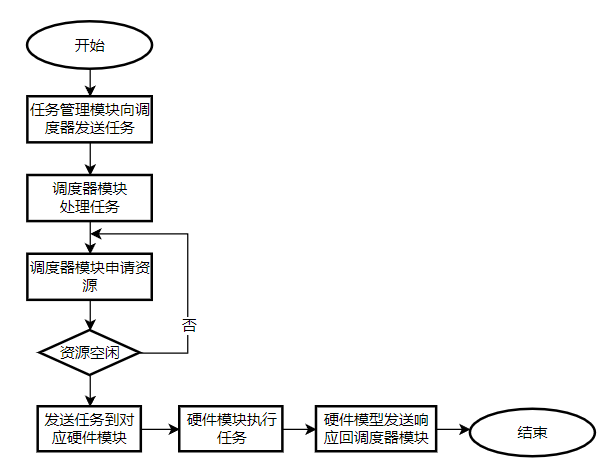
\includegraphics[width=0.8\textwidth]{任务执行流程图.png}
    \caption{任务执行流程图}
    \label{fig:badge}
\end{figure}

调度器模块需要将任务分发到调度器中资源调度模块申请的特定的硬件模型。
但由于整个平台软硬件设计分离,调度器模块无法获取硬件平台整体构
建信息,无法直接与硬件模块之间进行信息交互。因此我们需要一个模块实现调
度器模块与具体硬件模型之间的交互,为此我们在Processor模块中设
计了单实例ProcessorMgnt,用于实现消息交互功能。Processor模块以及
相关模块关系如图5.5所示:

\begin{figure}[!h]
    \centering
    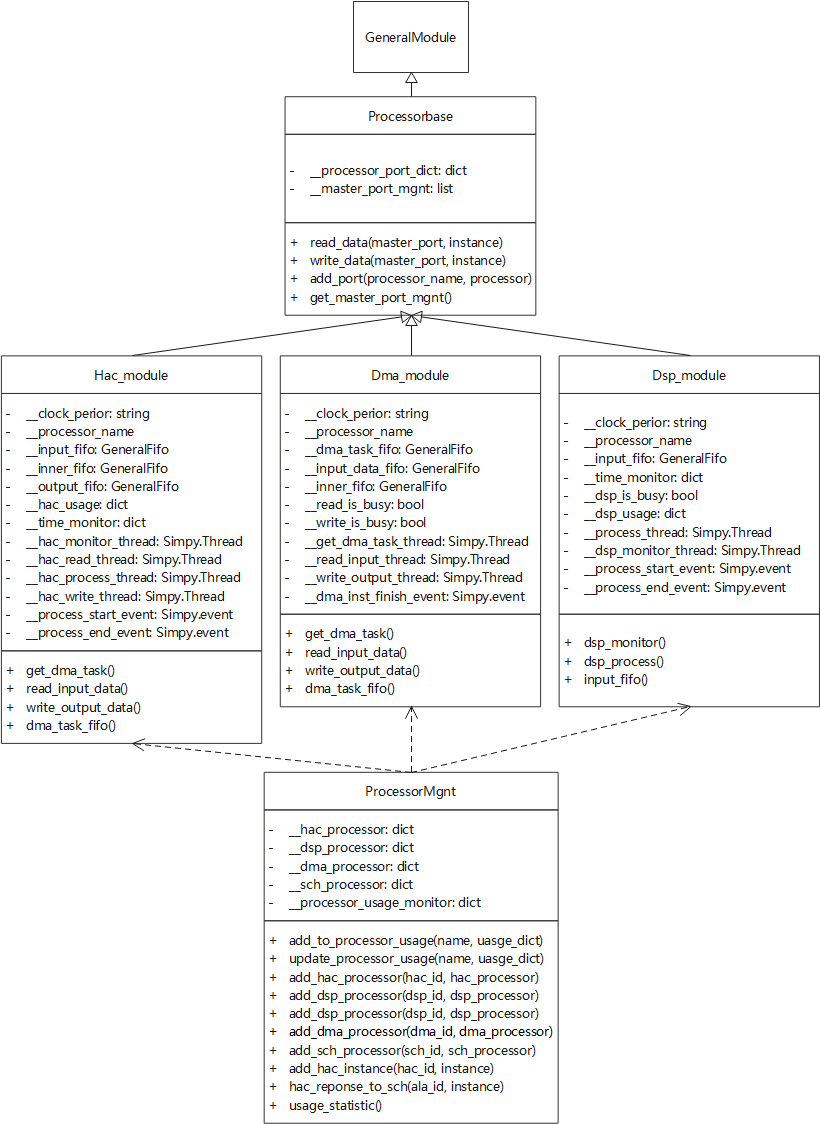
\includegraphics[width=0.8\textwidth]{Processor模块类图.png}
    \caption{Processor模块类图}
    \label{fig:badge}
\end{figure}

图5.5显示了ProcessorMgnt、三种具体的Processor模型、所有
Processor模型的基类ProcessorBase以及几者之间的关系。在
ProcessorMgnt模块中,各个模块在实例化的时候通过调用单实例的
对应方法通过相应类型的dict去记录,dict以模型名为键值。当其
他模块模块之间需要进行交互时,就可以通过调用ProcessorMgnt
单实例相应方法去访问对应字典,通过模型名就可以取到相应的模
型对象,从而进行交互。

三种基础的硬件模型以ProcessorBase为基类。ProcessorBase类实
现了几种基础硬件模型的公有方法:如实例化Port、读数据、写数
据、管理MasterPortMgnt等等。在介绍具体的Processor模型实现之前,
我们先介绍在仿真平台中传输的数据类型。

在仿真平台中传输的数据主要包括RwObject、Burst以及Flit三种。在
最外层硬件模块中传输数据的数据类型为RwObject,数据在总线上
传输的数据格式为Flit。这三种数据格式均包含着数据请求的关键信息:
请求类型、目的地址,数据长度等等,还包含着每个对象独有的id(如ObjectId,
BurstId等等)。DMA模块或者HAC模块需要进行数据搬运的时候,
将数据封装成RwObject发送到所在硬件对应的Port上,由PortMgnt模块
对RwObject进行拆分,将其拆封成总线位宽的Flit数据帧。Flit数据帧
仅在总线上可见,在仿真平台上可见的还是RwObject。图5.6为三种数据
类型的类图,以及图5.7为三种数据类型之间的关系图。
\\
\\
\\

\begin{figure}
    \centering
    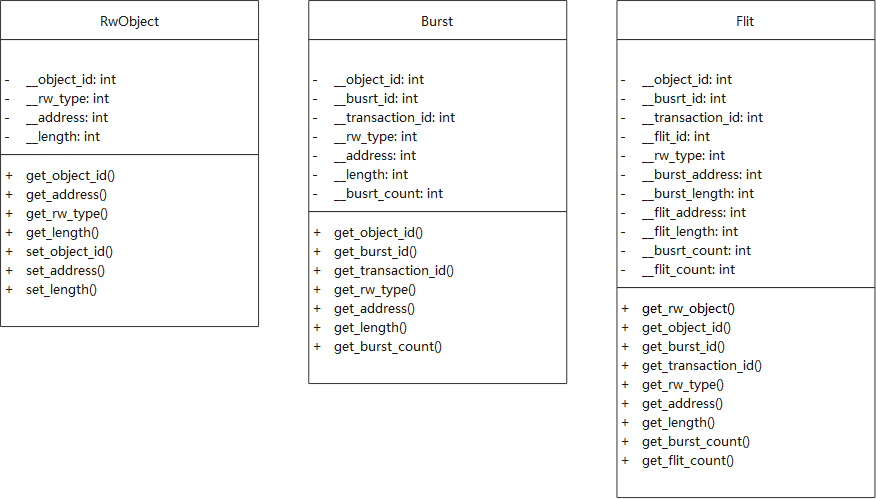
\includegraphics[width=1\textwidth]{三种数据类型类图.png}
    \caption{三种数据类型类图}
    \label{fig:badge}
\end{figure}

\begin{figure}
    \centering
    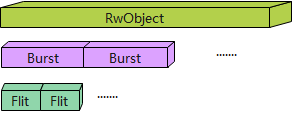
\includegraphics[width=0.6\textwidth]{数据类型关系图.png}
    \caption{数据类型关系图}
    \label{fig:badge}
\end{figure}


下面介绍三种基础硬件模型的具体实现:首先我们介绍DSP模块
的功能实现。DSP模块模拟的是DSP芯片的数据处理任务执行过程,在
仿真平台的流程中只需模拟真实的处理时延即可。调度器模块将任务用
例通过ProcessorMgnt模块发送到DSP模块的input\_fifo中,在硬件模
型中process\_thread一直在等待输入,DSP模型的input\_fifo中一旦有对象传入,
该事件被触发后,process\_thread进程就开始进行处理。处理时延在输入的任务
描述符中已经存在,DSP模型只需从任务描述符中取出时延信息,在乘以硬件的时钟
频率即可得到需要等待的仿真时间。DSP模块在任务链中作用负责完成输入数据的处理。
在仿真平台中只完成处理时延的仿真,并不真实的进行数据的处理。前搬移任务、DSP任
务以及后搬移任务形成一整个任务链,三者任务信息由同一个任务实例携带,当前搬移
DMA任务完成时,解析任务实例中的信息得到下一级DSP任务的硬件模型名,通过
ProcessorMgnt将任务实例发送到对应DSP模型input\_fifo中,触发相应的DSP任务,
发回调度器的响应只用来释放DMA任务申请的系统资源。

接下来介绍DMA模块的功能实现。在仿真平台中,DMA任务一般分为纯DMA任务、前搬移
任务以及后搬移任务。其中前搬移任务和后搬移任务都是包含在DSP任务链里面的,而
纯DMA任务只是单纯将数据从一块地址搬移到另外一块地址。DMA模块需要完成的对DSP
模块需要进行处理的数据的搬入搬出,将数据从对应SL2内存中搬入DSP模
块的PL2内存中的过程称为前搬移,将数据从PL2内存搬运到SL2
的过程称为后搬移。数据的搬入搬出,DMA模块通过任务用例中
的地址和数据大小信息创建RWObject,通过MasterPortMgnt经
过总线进行传输,DMA模块在实例化的过程中创建两个线程分别用来处理数据的搬入和
数据的搬出,以及创建一个线程获取DMA任务实例和控制总体
的流水线深度。DMA模块通过各级线程以及线程之间的Fifo实
现流水线。每一级线程均从Fifo中取出任务实例,执行完任务
实例之后,再将任务实例发到下一级线程的Fifo中,从而实现流水线
。DMA模块的流水线执行时序图如图5.8所示:

\begin{figure}
    \centering
    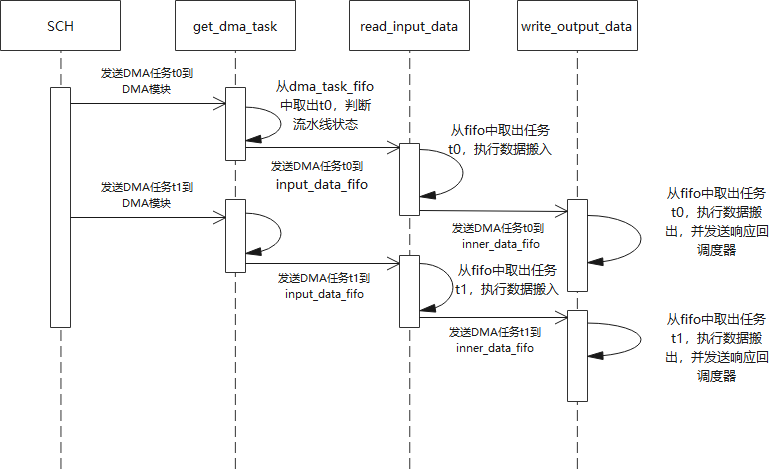
\includegraphics[width=1\textwidth]{DMA模块流水线时序图.png}
    \caption{DMA模块流水线时序图}
    \label{fig:badge}
\end{figure}


HAC模块是用来处理专用任务的硬件。一种HAC只用来执行一种任务,用来加速任务的处理。
HAC硬件模块中需要完成数据的搬入、处理以及搬出的一整套流程。HAC模块接收调度器
模块发送过来的HAC任务实例,HAC任务实例中记录着输入数据、处理时延以及输出数据等
相关信息。HAC模块通过三级流水实现数据搬入、数据处理以及数据搬出的功能。调度器模块
发送HAC任务实例到相应HAC模块的input\_fifo中,当input\_fifo接收到任务实例后,
HAC模块的input\_thread等待的事件被触发,进程加锁不再接收任务实例,进程开始执行
数据搬入的操作,把数据从相应的SL2内存中搬运到PL2内存中,操作执行结束后,将任务实例
放入inner\_fifo中,进程解锁。后续两个进程重复此类操作,形成HAC内部的三级流水的任务
执行。HAC模块的三级流水时序图如图5.9所示:

\begin{figure}
    \centering
    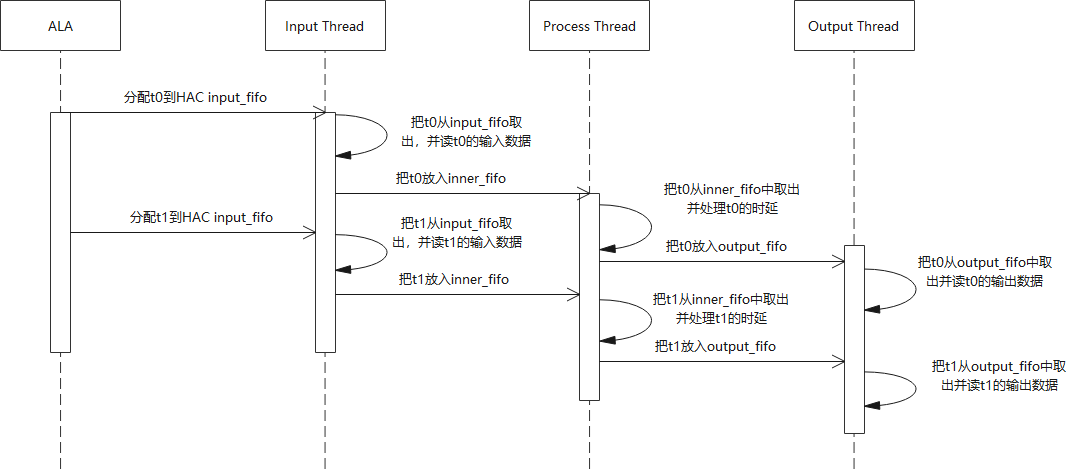
\includegraphics[width=1\textwidth]{HAC模块三级流水时序图.png}
    \caption{HAC模块三级流水时序图}
    \label{fig:badge}
\end{figure}

此外,Processor模块还在DSP模型和HAC模型中实现统计每个定长的时间片
内的硬件利用率。通过dsp\_monitor\_thread和hac\_monitor\_thread
两个进程分别去统计DSP模型和HAC模型的执行时间片。以DSP模块
为例,DSP模块在从FIFO中取出任务实例时触发process\_start\_event,
处理完时延后触发process\_end\_event。这两个事件都会使挂起的进程
开始执行,从而统计DSP模型每次执行的时间片区间。同时为了统计每一段
时间片内每个硬件的占用率,硬件模型中ProcessorMgnt模块统计了所有硬件模型的
对象,ProcessorMgnt模块在平台初始化时创建processor\_usage\_monitor字典,
processor\_usage\_monitor每个时间片的每个硬件模型的核利用率初始值设置为0,用于
统计每段时间片内的硬件利用率,并在对应的硬件模型中通过对应的进程去记录。在相应
的进程中,先设置变量Start和End来记录任务的开始时间戳以及结束时间戳,并设置标记
记录当前时间戳为任务开始的时间戳还是任务结束的时间戳。并通过每次Start和End之间时
间差去计算统计每个时间片的硬件利用率,并将相应的核利用率记录到processor\_usage\_monitor
中。在整个用例仿真结束后,在ProcessorMgnt模块中通过usage\_statistic方法去将
processor\_usage\_monitor中的内容统一的存储到数据库中。HAC模型内部工作时间块
统计与之相同。硬件模型核利用率的监控进程的伪代码如下所示:
\\
\\
\\
\\
\\
\begin{algorithm}[h]
    \renewcommand{\algorithmcfname}{伪代码}
    \caption{统计每个时间片内的核利用率}
    \KwData{时间片长度 $l$,任务开始时间戳 $Start$, 任务结束时间戳$End$, 当前时间戳类型$Flag$, 核利用率字典$processor\_usage\_dict$}
    \KwIn{进程触发时间戳 $time$}
    \KwResult{$processor\_usage\_dict$}
    \BlankLine
    $Start$ \leftarrow 0\;
    $End$ \leftarrow 0\;
    \tcc{loops}
    \emph{the thread is triggered}\;
    \tcp{$Flag$(0: the $time$ is start; 1:the $time$ is end)}
    \If{$Flag$ is 0}{
        $k$ \leftarrow $End$ / $l$\;
        $interval$ \leftarrow ($time$ - $k*l$)\;
        $n$ \leftarrow $interval$ / $l$\;
        \If{$n != 0$}{
            \For{$i=k+1$ \KwTo $k+n$}{
                $processor\_usage\_dict$(i) \leftarrow $0$\;  
            }
        }
        $Start$ \leftarrow $time$\;
        $Flag$ \leftarrow $1$\;
    }
    \Else{
        $k$ \leftarrow $Start / l$\;
        $interval$ \leftarrow $(time - k*l)$\;
        $n$ \leftarrow $interval$ / $l$\;
        \If{$n!=0$}{
            $processor\_usage\_dict(k)$ \leftarrow ($processor\_usage\_dict(k) + (k*l - Start)/l$)\;
            \If{$n != 1$}{
                \For{$i=k+1$ \KwTo $k+n-1$}{
                    $processor\_usage\_dict(k+1)$ \leftarrow $1$;
                }
            }
            $processor\_usage\_dict(k+1)$ \leftarrow $(time - (k+1)*l)/l$\;
        }
        \Else{
            $processor\_usage\_dict(k+1)$ \leftarrow $(time - Start)/l$\;
        }
        $End$ \leftarrow $time$\;
        $Flag$ \leftarrow $0$\;
    }
\end{algorithm}

\section{仿真平台Memory模块设计与实现}

仿真平台的Memory模块主要实现接收Master设备通过总线互联模块发送
过来的读写请求flit,根据Bank位宽拆成对应的Bank操作发送到对应地
址的Bank的FIFO上。

Memory模块提供交织的Bank。这些Bank模块根据地址相互交织,每个Bank
的偏移地址与Bank位宽相同。仿真平台中Memory模块Bank模块设计为4个Bank,
Bank位宽为256字节的设计方案。Memory模块在实例化的时候创建4个Bank模块,
Memory模块可以同时处理不同的Bank模块上的Bank操作,但每个Bank模块同时只
能处理一个Bank操作。Bank模块的交织方案如图5.10所示:
\\
\begin{figure}
    \centering
    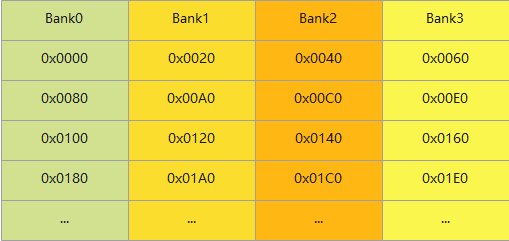
\includegraphics[width=0.82\textwidth]{Bank模块交织方案.png}
    \caption{Bank模块交织方案}
    \label{fig:badge}
\end{figure}

Bank模块在初始化时创建读写Bank线程。读写Bank操作完成向对应的SlavePort
发送读写响应flit。Memory模块接收SlavePort发送过来的flit,因为对读写请
求的操作不同,Memory模块会根据读写请求的区别分到不同的FIFO中。Memory对
发送过的flit的处理流程图如图5.11所示:

\begin{figure}
    \centering
    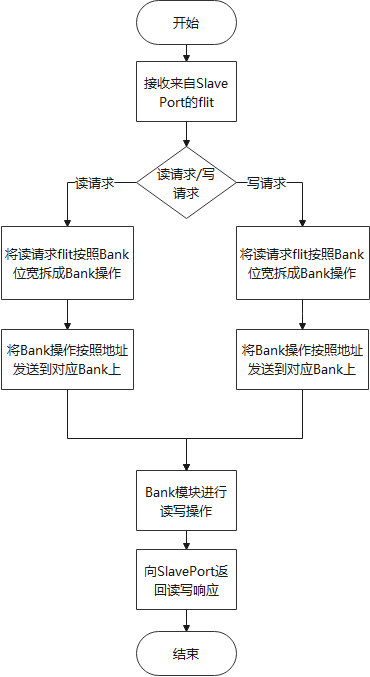
\includegraphics[width=0.49\textwidth]{Memory模块处理流程图.png}
    \caption{Memory模块处理流程图}
    \label{fig:badge}
\end{figure}

Bank写操作结束时,Memory模块会统计一个Burst完成flit的数量,当最后一个flit
操作完成后会统一发送一个写响应回SlavePort。而Bank读操作则时完成一个flit就
发送一个flit的读响应到SlavePort上。最后由总线互联模块发送回发送读写请求的
Master设备,完成一整个读写操作。

\section{设计空间探索相关模块的设计与实现}

设计空间探索模块实现的功能是对我们所需要探索的设计目标在设计空间中寻找最优
或者是较优设计。设计空间模块主要分为三个模块:训练集生成模块、预测模型生成
模块以及遗传算法探索模块。设计空间探索模块的整体流程图如图5.12所示:

\begin{figure}
    \centering
    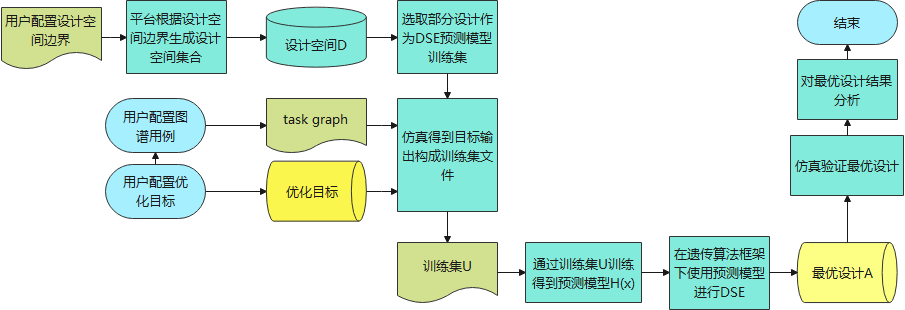
\includegraphics[width=1\textwidth]{设计空间探索模块整体流程图.png}
    \caption{设计空间探索模块整体流程图}
    \label{fig:badge}
\end{figure}

接下来主要介绍训练集生成模块和预测模型生成模块的具体设计与实现以及设计空间探索结果分析。

\subsection{训练集生成模块的设计与实现}

训练集生成模块主要包括设计参数、设计边界与目标值的选取、设计空间的生成以及根据设计空间
以及目标值生成下一步预测模型所需要的训练集文件。在仿真平台中我们选取可配置参数作为我们
的设计参数,并根据实际情况设置各个设计参数的设计边界,具体设计参数及设计边界如表5.1所示:

\begin{table}[!h]
    \centering\normalsize
    \caption{仿真平台设计空间}
    \begin{tabular}{c|c|c}
    \hline
    \textbf{设计参数} & \textbf{设计参数取值}         & \textbf{数量} \\ \hline
    PL2 Pool Size & 100000-190000: 10000+   & 19          \\ \hline
    PL2 Unit Size & 10-50: 10+              & 5           \\ \hline
    SL2 Pool Size & 1500000-1850000: 50000+ & 7           \\ \hline
    SL2 Pool Size & 10-50: 10+              & 5           \\ \hline
    Cu Num        & 1-5: 1+                 & 5           \\ \hline
    Dsp Num       & 4-16: 2+                & 7           \\ \hline
    BUS Bit Width & 64-512: 64+             & 8           \\ \hline
    \end{tabular}
    \end{table}

我们选取了七个参数作为我们设计空间探索的设计参数值,设计参数分别为:PL2内存池大小、PL2每个内存单元大小、SL2内存池大小、SL2每个内存单元大小、Cu数量、Dsp数量以及总线位宽。这些参数均会影响最后仿真结果。这些设计参数的组合最后构成的设计空间包括了超过56万个不同的设计配置。

我们设计空间探索主要探索的方向主要是时延以及核的使用方面。我们最终选取了仿真时延、每个TTI核的利用率、每个TTI核的一致性为我们设计空间探索的目标值。接下来我们说明每个目标值的统计标准。仿真时延在数据库文件中有着直接的记录,我们只需直接提取数据库中的信息即可,核的利用率在数据库中记录了每个时间片(0.002TTI)的核的利用率,记录方法已在5.1.5节介绍。我们只需将数据库中信息整合每个TTI的核的利用率即可。核的一致性指的是在同个TTI内所有核的利用率的方差,我们需要将之前统计的核的利用率进行计算即可。这就是我们设计空间探索的优化目标值。

我们生成训练集的流程图如图4.9所示。我们将RatConfig表中需要改变的参数值单独设置一页Config
表,并将这一页的值与整张表中的相关的值相关联,通过openpyxl插件去修改Config表中的参数。
这样我们就可以通过脚本自动改变设计参数去运行仿真,仿真结束后提取数据库中目标值信息,处理
后将设计参数和目标值一同输出到训练集文件中。我们训练集文件大小为6000,生成训练集模块一共
运行了6000次仿真。训练集文件格式如图5.13所示:

\begin{figure}
    \centering
    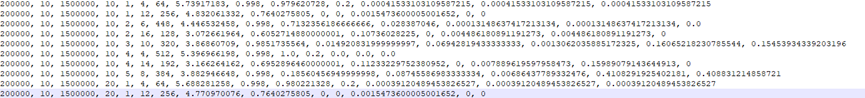
\includegraphics[width=1\textwidth]{训练集文件格式示例.png}
    \caption{训练集文件格式示例}
    \label{fig:badge}
\end{figure}

\subsection{预测模型生成模块设计与实现}

我们在遗传算法进行设计空间探索过程中,在不断迭代每一代种群时如果每一次都要进行仿真从而得到对应设计参数的目标值,整体设计空间探索的时间就会十分的漫长。于是,我们使用机器学习生成的预测模型去代替实际的仿真平台去进行遗传算法设计空间探索的过程,这样能够大大减少设计空间探索的时间。

我们多目标预测模型采用先对不同目标值分别进行机器学习的过程,得到对应7个目标值的7个预测模型。我们将这7个预测模型通过一个multi\_model类集成到一起,通过multi\_model类的方法我们可以通过输入设计参数从而得到相应的目标值。多目标预测模型集成的各个目标值的准确度(以R2确定系数为标准)如表5-2所示:

\begin{table}[!h]
    \centering\normalsize
    \caption{多目标预测模型误差值}
    \begin{tabular}{|c|c|c|c|}
    \hline
    \textbf{时延}       & \textbf{TTI0核利用率} & \textbf{TTI1核利用率} & \textbf{TTI2核利用率} \\ \hline
    0.99824568        & 0.9999998         & 0.9982341         & 0.9873023         \\ \hline
    \textbf{TTI0核一致性} & \textbf{TTI1核一致性} & \textbf{TTI2核一致性} & \textbf{}         \\ \hline
    0.8638929         & 0.9831229         & 0.8559540         &                   \\ \hline
    \end{tabular}
    \end{table}

从表中我们可以清楚的看出对于多个目标值而言,每个目标值的误差值不超过0.15。整个预测模型可以
比较高效精准的预测出目标值,与真实仿真平台的仿真结果相差不大,为了更加精准的看出预测模型
与仿真平台的结果差距,我们将1200次仿真结果作为验证集与预测模型进行对比,仿真结果与预测结果
对比如图5.14所示:

\begin{figure}[!h]
    \centering
    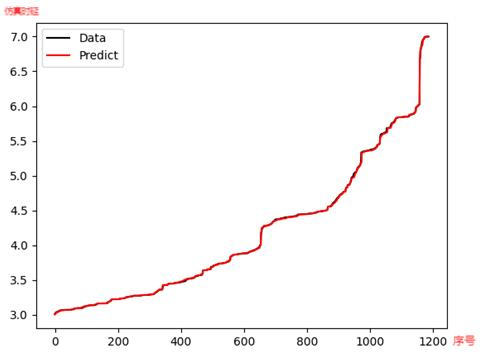
\includegraphics[width=0.45\textwidth]{仿真结果与预测结果对比图1.png}
\end{figure}

\begin{figure}[!h]
    \centering
    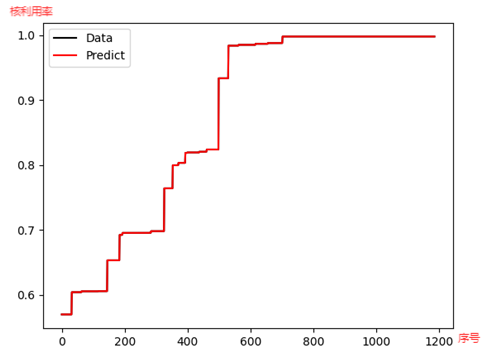
\includegraphics[width=0.45\textwidth]{仿真结果与预测结果对比图2.png}
\end{figure}

\begin{figure}[!h]
    \centering
    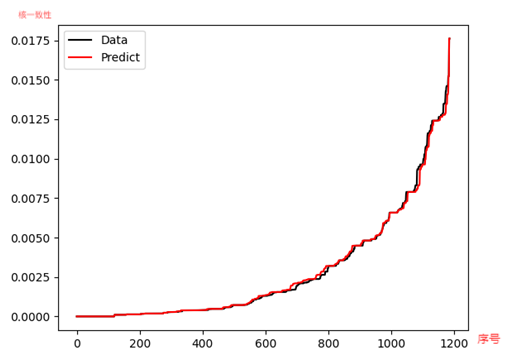
\includegraphics[width=0.45\textwidth]{仿真结果与预测结果对比图3.png}
    \caption{仿真结果与预测结果对比图}
\end{figure}

\subsection{设计空间探索结果分析}

在得到多目标预测模型之后,我们将使用多目标预测模型使用遗传算法进行设计空间探索。遗传算法执行过程中我们
使用NGSA-Ⅱ,我们通过交叉变异等操作产生子代,将父代和子代放到一起进行快速非支配排序,构造出不同等级
的非支配解集。按照需求计算每一代所有个体的拥挤距离,并根据拥挤度比较构造下一代种群。

遗传算法我们遗传代数设置为200代,每代种群数量为50,变异概率为0.1。最终演化种群中的每个基因型经过仿真平
台仿真运行得出相应的目标值。最终我们得到了50个设计方案,并且将这50个设计方案在仿真平台上进行仿真,得到
了相应的目标值。我们根据这50个设计方案以及对应的目标值进行探索,得到了以下结论。

我们先将三个方面的50个目标值与原始设计相对比得到图5.15。

\begin{figure}
    \centering
    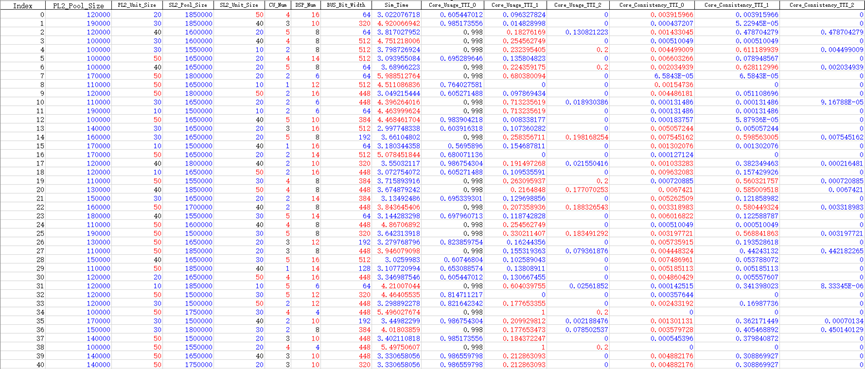
\includegraphics[width=1\textwidth]{设计空间探索结果仿真目标值结果对比图.png}
    \caption{设计空间探索结果仿真目标值结果对比图}
    \label{fig:badge}
\end{figure}

根据图5.15针对仿真时延、核利用率以及核一致性三个目标值,我们可以得到相
对于这三个目标值各自方向的最优解。下面我们对三个目标值单独进行分析并将
设计空间探索所得到的最优解集放在一起进行比较。我们基于优化目标将所有方
案的结果以及原始设计方案放到一起进行比较。比较结果如图5.16至5.18所示:

\begin{figure}[h]
    \centering
    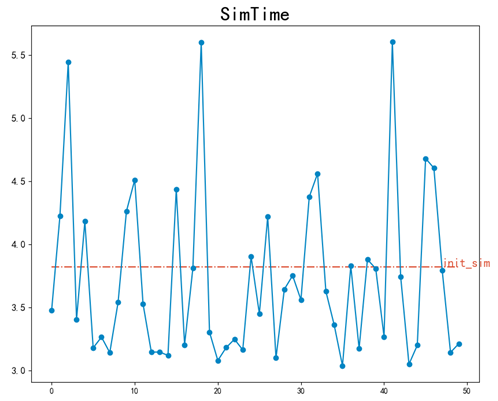
\includegraphics[width=0.53\textwidth]{50组设计方案时延结果对比.png}
    \caption{50组设计方案时延结果对比}
    \label{fig:badge}
\end{figure}

图5.16中横坐标为设计方案序号,纵坐标为仿真时延,红色虚线为初始设计方案及其对应的仿真时延。
由图5.16及对应序号的设计方案可以看出序号为35、43、20、27、14、7、48、12、13、23的方案较好。并且通过各个设计方案值之间的结果对比可以得出影响时延结果的主要因素为核的数量以及总线位宽等等。
\begin{figure}[h]
    \centering
    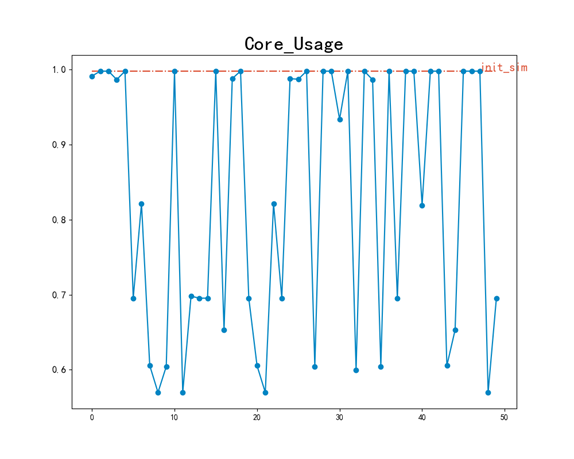
\includegraphics[width=0.6\textwidth]{50组设计方案核利用率结果对比.png}
    \caption{50组设计方案核利用率结果对比}
    \label{fig:badge}
\end{figure}

由图5.17及对应序号的设计方案可以看出序号33、28、42、29、47、39、36、38、4、26的方案较好。
并且通过各个设计方案之间的结果对比可以得出影响核利用率的主要因素为核的数量及CU数量等等。

\begin{figure}[h]
    \centering
    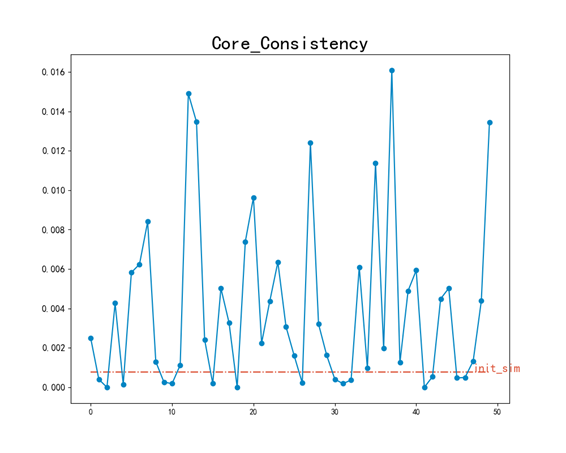
\includegraphics[width=0.6\textwidth]{50组设计方案核一致性结果对比.png}
    \caption{50组设计方案核一致性结果对比}
    \label{fig:badge}
\end{figure}

由图5.18及对应序号的设计方案可以看出序号2、18、41、4、31、15、10、26、9、32的方案较好。
并且通过各个设计方案之间的结果对比可以得出影响核利用率的主要因素为核的数量及CU数量等等。
而且对比图5.16和图5.17可以发现核利用率和核一致性的优化方向和影响因素大致相同。

但针对多个目标值同时考虑而言,我们需要找到多个目标值均衡的几个设计方案。从图5.16至图5.18可以看出
时延和核的利用率优化方向相反。仿真时延低的几种方案,设计参数中Dsp数量较大,但由于Dsp数量较大,
导致核的利用率和一致性效果较差。而核的利用率和核的一致性优化方向相同,最优的几个设计方案设计参数
大致相同。于是我们就核利用率和仿真时延两个方面进行考虑,结果图如图5.19所示:
\\
\\
\begin{figure}[h]
    \centering
    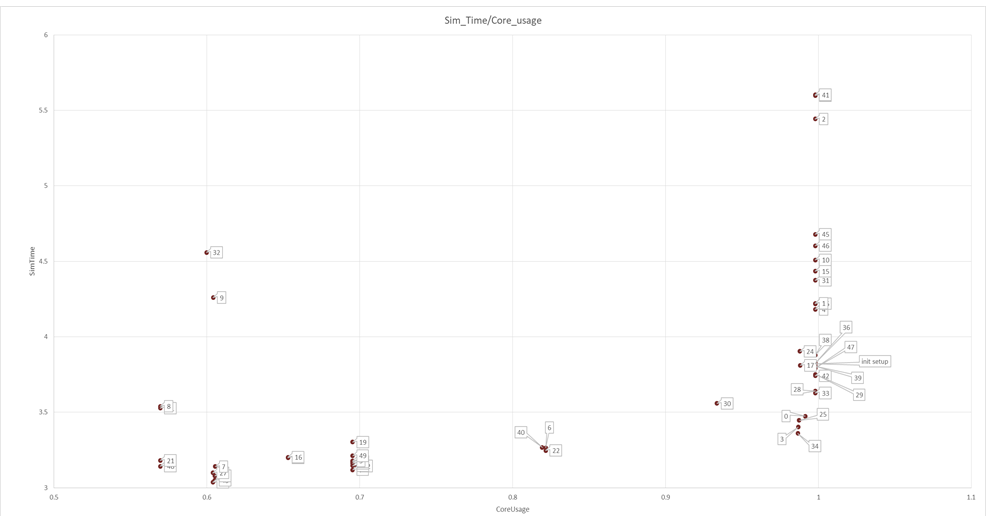
\includegraphics[width=1\textwidth]{仿真平台结果分析图.png}
    \caption{仿真平台结果分析图}
    \label{fig:badge}
\end{figure}

从图5.19中我们可以找到6种方案在仿真时延和核利用率两个方面表现都很优秀的设计方案如表5.3所示:

\begin{table}[h]
    \centering\footnotesize
    \caption{最优设计方案设计参数}
    \begin{tabular}{|c|c|c|c|c|c|c|c|}
    \hline
    Index & PL2\_Pool\_Size & PL2\_Unit\_Size & SL2\_Pool\_Size & SL2\_Unit\_Size & Cu\_Num & Dsp\_Num & BUS\_Bit\_Width \\ \hline
    33    & 140000          & 30              & 1550000         & 20              & 4       & 8        & 448             \\ \hline
    25    & 170000          & 40              & 1650000         & 10              & 5       & 10       & 320             \\ \hline
    3     & 170000          & 20              & 1800000         & 50              & 2       & 10       & 512             \\ \hline
    42    & 100000          & 20              & 1800000         & 20              & 4       & 8        & 512             \\ \hline
    0     & 100000          & 10              & 1750000         & 50              & 4       & 10       & 128             \\ \hline
    25    & 170000          & 30              & 1650000         & 10              & 5       & 10       & 320             \\ \hline
    \end{tabular}
    \end{table}

从整体设计参数以及目标值的变化,我们可以看出增加Cu数量可以增快仿真速度,提高总线带宽可以使核的利用率提高同时还可以增快仿真速度。

\section{本章小结}

本章的工作主要是在第四章概要设计的基础上,详细的阐述了仿真平台中硬件平台
的构建、Processor模块以及Memory模块的具体实现,介绍了设计空间探索流程的
具体设计和实现。实现整个仿真平台的搭建以及基于仿真平台的设计空间探索流程,
最后得到了设计空间探索结果种群,并对最终得到的设计空间探索结果进行了分析,得到了最终的
最优设计方案以及设计方案优化的目标

在本章基础上,下一章节我们将完成对仿真平台的测试。